\chapter{Validación}\label{cap:validacion}

\section{Introducción}

Este capítulo presenta la validación experimental de los dos enfoques implementados: el baseline clásico MFCC + SVM y el enfoque profundo basado en MERT congelado y SVM. Se recogen la ejecución de los experimentos, la selección de configuraciones, la evaluación final en \textit{test}, la comparación predictiva y operacional, y la selección del modelo para la prueba de concepto web.

\section{Baseline MFCC + SVM}

\subsection*{Configuración y selección}

El baseline procesó los 1\,000 ejemplos del manifiesto experimental sin registrar fallos.

La búsqueda de hiperparámetros evaluó 16 configuraciones de SVM RBF, combinando $C \in \{0{,}1;\ 1;\ 10;\ 100\}$ y $\gamma \in \{\textit{scale};\ 0{,}001;\ 0{,}01;\ 0{,}1\}$. La configuración seleccionada fue $C=10$ y $\gamma=0{,}01$, ajustada con \textit{train} y seleccionada con \textit{val}.

\subsection*{Resultados}

\begin{table}[H]
    \centering
    \resizebox{\textwidth}{!}{%
    \begin{tabular}{lrrrrr}
        \hline
        \textbf{Partición} & \textbf{Balanced accuracy} & \textbf{Precision IA} & \textbf{Recall IA} & \textbf{F1 IA} & \textbf{ROC-AUC} \\
        \hline
        \textit{val} & 0,7800 & 0,7625 & 0,8133 & 0,7871 & 0,8480 \\
        \textit{test} & 0,8333 & 0,8472 & 0,8133 & 0,8299 & 0,9086 \\
        \hline
    \end{tabular}
    }
    \caption{Medidas predictivas del baseline MFCC + SVM en \textit{val} y \textit{test}.}
    \label{tab:mfcc-svm-resultados}
\end{table}

En \textit{test}, el baseline obtiene 125 aciertos sobre 150 ejemplos. La matriz de confusión muestra que clasifica correctamente 64 de los 75 ejemplos humanos y 61 de los 75 ejemplos IA, con 11 falsos positivos y 14 falsos negativos. Esta distribución indica una dificultad ligeramente mayor para reconocer la clase IA, coherente con un recall humano de 0,8533 y un recall IA de 0,8133. La Figura~\ref{fig:mfcc-svm-confusion} recoge esta distribución de aciertos y errores.

\begin{figure}[H]
    \centering
    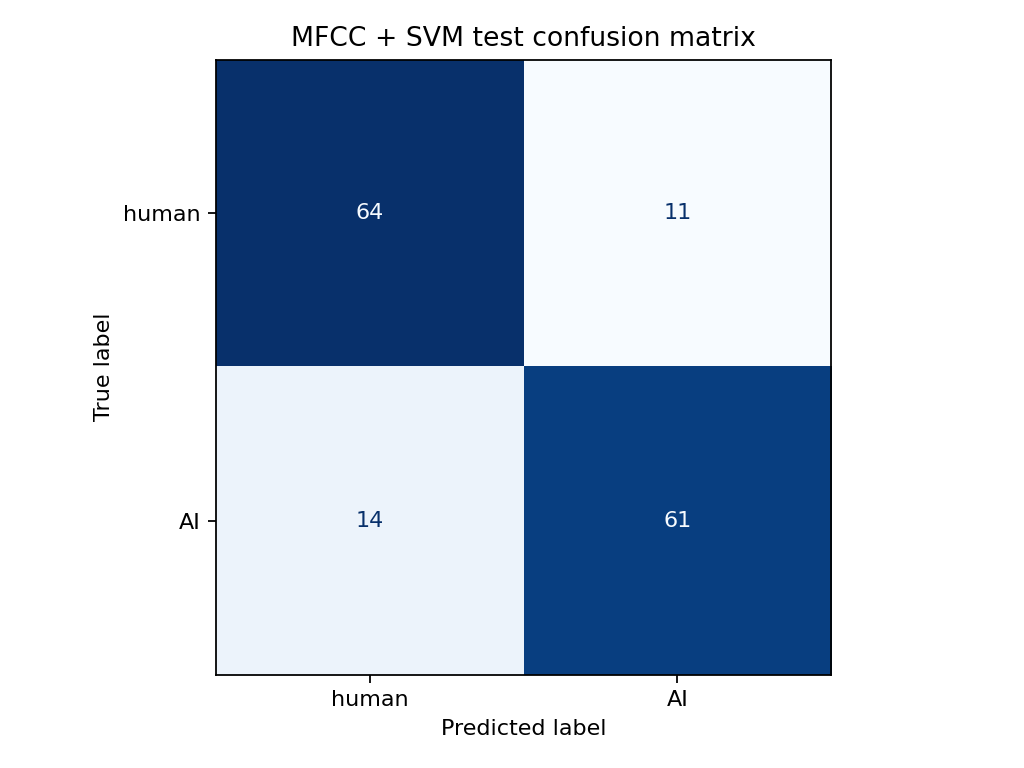
\includegraphics[width=0.72\textwidth]{fig/mfcc_svm_confusion_matrix.png}
    \caption{Matriz de confusión del baseline MFCC + SVM en \textit{test}.}
    \label{fig:mfcc-svm-confusion}
\end{figure}

\section{MERT congelado + SVM}

\subsection*{Extracción de embeddings}

Antes de procesar el subconjunto completo se ejecutó un smoke test técnico en CPU. Esta prueba verificó las dimensiones de entrada y salida, la presencia de valores finitos, el determinismo de la extracción y la viabilidad de ejecución en CPU.

La extracción completa procesó los 1\,000 ejemplos del manifiesto sin fallos, IDs ausentes ni duplicados. Cada clip produjo un vector de 768 componentes y el conjunto completo quedó representado mediante una matriz de forma $(1000, 768)$. Los embeddings se almacenaron como float32 y sus metadatos se verificaron frente al manifiesto.

\subsection*{Selección del clasificador}

El clasificador sobre embeddings se construyó como un pipeline \textit{StandardScaler} + SVM. Se evaluaron candidatos con kernel lineal y RBF. Todos los candidatos se ajustaron con \textit{train} y se seleccionaron con \textit{val}. La regla de selección maximizó \textit{balanced accuracy}; en caso de empate, consideró ROC-AUC, F1 de la clase IA, menor latencia media de predicción y preferencia por kernel lineal. La configuración seleccionada fue una SVM lineal con $C=0{,}1$. Las medidas obtenidas por esta configuración en \textit{val} se recogen en la Tabla~\ref{tab:mert-svm-validacion}.

\begin{table}[H]
    \centering
    \resizebox{\textwidth}{!}{%
    \begin{tabular}{lrrrrr}
        \hline
        \textbf{Modelo} & \textbf{Balanced accuracy} & \textbf{Precision IA} & \textbf{Recall IA} & \textbf{F1 IA} & \textbf{ROC-AUC} \\
        \hline
        MERT + SVM lineal & 0,8667 & 0,8395 & 0,9067 & 0,8718 & 0,9218 \\
        \hline
    \end{tabular}
    }
    \caption{Medidas de \textit{val} del clasificador seleccionado sobre embeddings MERT.}
    \label{tab:mert-svm-validacion}
\end{table}

\subsection*{Resultados}

Una vez fijada la configuración mediante \textit{val}, el enfoque basado en MERT se evaluó en \textit{test} utilizando los embeddings precomputados y una SVM lineal con $C=0{,}1$. La Tabla~\ref{tab:mert-svm-test} recoge las medidas obtenidas.

\begin{table}[H]
    \centering
    \resizebox{\textwidth}{!}{%
    \begin{tabular}{lrrrrr}
        \hline
        \textbf{Modelo} & \textbf{Balanced accuracy} & \textbf{Precision IA} & \textbf{Recall IA} & \textbf{F1 IA} & \textbf{ROC-AUC} \\
        \hline
        MERT + SVM lineal & 0,8200 & 0,8158 & 0,8267 & 0,8212 & 0,8985 \\
        \hline
    \end{tabular}
    }
    \caption{Medidas de \textit{test} de MERT + SVM lineal.}
    \label{tab:mert-svm-test}
\end{table}

En \textit{test}, el enfoque basado en MERT obtuvo 123 aciertos sobre 150 ejemplos. Clasificó correctamente 61 de los 75 ejemplos humanos y 62 de los 75 ejemplos IA, con 14 falsos positivos y 13 falsos negativos. La distribución de errores entre ambas clases fue prácticamente equilibrada, como muestra la Figura~\ref{fig:mert-svm-confusion}.

\begin{figure}[H]
    \centering
    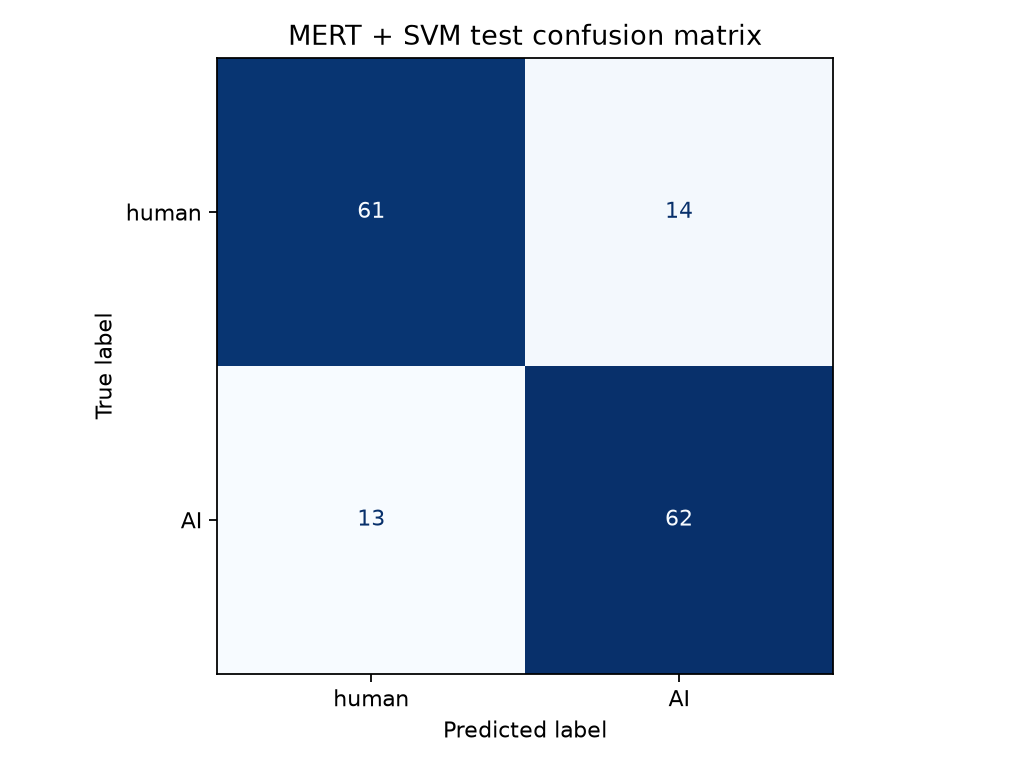
\includegraphics[width=0.72\textwidth]{fig/mert_svm_test_confusion_matrix.png}
    \caption{Matriz de confusión de MERT + SVM lineal en \textit{test}.}
    \label{fig:mert-svm-confusion}
\end{figure}

\section{Comparación y selección del modelo}

\subsection*{Comparación predictiva}

La Tabla~\ref{tab:comparacion-test} presenta las medidas de \textit{test} de ambos enfoques y la diferencia MERT menos MFCC.

\begin{table}[H]
    \centering
    \resizebox{\textwidth}{!}{%
    \begin{tabular}{lrrrrr}
        \hline
        \textbf{Modelo} & \textbf{Balanced accuracy} & \textbf{Precision IA} & \textbf{Recall IA} & \textbf{F1 IA} & \textbf{ROC-AUC} \\
        \hline
        MFCC + SVM RBF & 0,8333 & 0,8472 & 0,8133 & 0,8299 & 0,9086 \\
        MERT + SVM lineal & 0,8200 & 0,8158 & 0,8267 & 0,8212 & 0,8985 \\
        Diferencia MERT - MFCC & -0,0133 & -0,0314 & +0,0133 & -0,0087 & -0,0101 \\
        \hline
    \end{tabular}
    }
    \caption{Comparación predictiva en \textit{test}.}
    \label{tab:comparacion-test}
\end{table}

La Tabla~\ref{tab:comparacion-errores} compara los aciertos y errores principales de ambos enfoques.

\begin{table}[H]
    \centering
    \begin{tabular}{lrrr}
        \hline
        \textbf{Modelo} & \textbf{Aciertos} & \textbf{Falsos positivos} & \textbf{Falsos negativos} \\
        \hline
        MFCC + SVM RBF & 125 & 11 & 14 \\
        MERT + SVM lineal & 123 & 14 & 13 \\
        Diferencia MERT - MFCC & -2 & +3 & -1 \\
        \hline
    \end{tabular}
    \caption{Comparación de aciertos, falsos positivos y falsos negativos en \textit{test}.}
    \label{tab:comparacion-errores}
\end{table}

En \textit{test}, los resultados de ambos enfoques fueron próximos y deben interpretarse como comparables dentro de AIME. MFCC + SVM alcanzó una ligera ventaja en \textit{balanced accuracy}, precision IA, F1 IA y ROC-AUC, además de obtener 125 aciertos frente a los 123 del enfoque profundo. MERT + SVM presentó un recall IA ligeramente superior y un falso negativo menos. Dado el reducido tamaño de las diferencias observadas, estos resultados no permiten afirmar una superioridad estadísticamente significativa de MFCC sobre MERT. Las diferencias se circunscriben al \textit{test} de AIME empleado en el experimento.

\subsection*{Comparación operacional}

La comparación operacional de la Tabla~\ref{tab:comparacion-operacional} se refiere al clasificador aplicado sobre representaciones ya calculadas. En el baseline se usan características MFCC ya extraídas, mientras que en el enfoque profundo se usan embeddings MERT ya extraídos. El tamaño corresponde al clasificador serializado; en el caso de MERT no incluye el processor ni el encoder.

\begin{table}[H]
    \centering
    \begin{tabular}{lrr}
        \hline
        \textbf{Modelo} & \textbf{Latencia (ms/ejemplo)} & \textbf{Tamaño (MB)} \\
        \hline
        MFCC + SVM RBF & 0,090 & 0,14 \\
        MERT + SVM lineal & 0,113 & 1,69 \\
        \hline
    \end{tabular}
    \caption{Comparación operacional de los clasificadores.}
    \label{tab:comparacion-operacional}
\end{table}

Las latencias de 0,090 y 0,113 ms por ejemplo proceden de una única temporización sobre los 150 ejemplos de \textit{test}; en ambos casos, la latencia se obtuvo dividiendo el tiempo total de la predicción y de la obtención de los \textit{decision scores} entre 150. Estas mediciones cubren únicamente los clasificadores sobre representaciones previamente calculadas: las 40 características MFCC y los embeddings MERT de 768 dimensiones, respectivamente. No se registraron repeticiones independientes ni un \textit{warm-up}, por lo que se utilizan solo como referencia operacional y no como un benchmark riguroso. Por su parte, el tiempo aproximado de 0,824 s por clip de MERT corresponde a la media de los pases del encoder sobre los 1\,000 clips procesados en CPU, con tamaño de lote 1 y dos ventanas de cinco segundos por clip; no incluye decodificación, preparación con el \textit{processor}, \textit{pooling} ni escritura, por lo que tampoco constituye una medición extremo a extremo.

La diferencia entre las latencias de los clasificadores es pequeña y no debe interpretarse como una ventaja temporal fuerte entre los pipelines completos. La ejecución de MERT requiere además el \textit{processor}, el encoder profundo y las dependencias de aprendizaje profundo, mientras que los 1,69 MB informados corresponden solo a \textit{StandardScaler} + SVM y no al pipeline MERT completo. Por tanto, la evidencia operacional disponible es parcial: el clasificador serializado de MFCC ocupa menos espacio y su pipeline requiere menos componentes, pero las mediciones presentadas no comparan de forma homogénea la ejecución completa de ambos enfoques.

\subsection*{Selección}

Las configuraciones de ambos enfoques se seleccionaron con \textit{train} y \textit{val}, y \textit{test} se reservó para una única evaluación final comparativa. Una vez observados esos resultados, la elección del modelo integrado en la aplicación web se realizó como una decisión de ingeniería, sin reajustar hiperparámetros utilizando \textit{test}.

MFCC + \textit{StandardScaler} + SVM RBF fue seleccionado como modelo para VeriSon. Los dos enfoques presentan un rendimiento similar dentro del \textit{test} de AIME, por lo que esta decisión no implica haber demostrado una superioridad científica concluyente de MFCC. Para el MVP, MFCC ofrece una combinación más favorable desde el punto de vista de la integración y el despliegue: su pipeline es más simple, no requiere ejecutar un encoder profundo durante la inferencia, incorpora menos dependencias y presenta una menor complejidad operacional. Su clasificador serializado también es más pequeño; en cambio, el tamaño informado para MERT corresponde solo a \textit{StandardScaler} + SVM y no incluye el encoder ni las dependencias adicionales necesarias para el pipeline profundo completo.
